\section{Evaluation}
\label{sec:eval}

We've evaluated Tutamen in a variety of scenarios using the
applications described in \S~\ref{sec:apps}. In this section, we
discuss both our existing Tutamen deployment as well as the
performance characteristics of out Tutamen prototype.

\subsection{Deployment}
\label{sec:eval:deployment}

We've deployed a group of Tutamen servers, each either hosted locally
or by an independent third party in order to gain geospatial,
geopolitical, and administrative diversity. Our current Tutamen
deployment includes three access control and storage server
pairs\footnote{In each instance, both an Access Control Server and a
  Storage Server run on single virtual or physical machine in order to
  simplify the deployment process. If desired, these roles could be
  separate for performance purposes.}:

\begin{packed_desc}
\item[Paris, France:] Scaleway~\cite{scaleway} C2S instance (bare
  metal, 4-core, 8GB, Intel Atom C2550).
\item[North Virginia:] AWS EC2~\cite{amazon-ec2} c4.large instance
  (VM, 2-core, 3.75GB, Intel Xeon E5-2666).
\item[Boulder, CO:] Self-hosted instance (VM, 4-core, 4GB virtual,
  Intel Xeon E3-1245).
\end{packed_desc}

We are able to use this test deployment to shard secrets across all
three storage servers and all three access control servers. By
default, the Tutamen CLI utility shards a secret across all available
storage servers with no redundancy (i.e. $n=k=\#_{SS}$) and requires
the approval of each AC control server to read each shard of the
secret (i.e. $n=k=\#_{ACS}$). Thus, by default, the CLI will shard
each secret via $n=k=3$ across each storage and access control
server. This arrangement provides no redundancy, but also requires the
minimal level of trust of each individual Tutamen server and hosting
provider. The sharding value of $n$ and $k$ for both storage and
access control servers can be specified individually for each secret
collection, however, so it is trivial for individual Tutamen
applications and users to set these values as they desire.

We've utilized our experimental Tutamen deployment to manually store
secrets via the Tutamen CLI, to store encryption keys for our FuseBox
app, and to store encryption keys for our LUKS and our QCOW2 full-disk
encryption systems. All of these scenarios share the quality that they
require a low rate of secret storage/retrieval requests. E.g. FuseBox
requires only a single secret store per file create operation and a
single secret lookup per file open operation. The full disk encryption
schemes are even less demanding, requiring only a single lookup per
system boot. Thus, we have not yet had a need to optimize our Tutamen
deployment for performance (see \S~\ref{sec:eval:perf}). Our current
deployment has easily supported the needs of our existing Tutamen
users and applications. This deployment demonstrates Tutamen's
usefulness as an enabler of previously unattainable functionally in a
manner that also minimizes the need for third party trust. While
Tutamen is still a prototype, our experience utilizing it thus far
leads us to believe it provides a well-designed architecture capable
of supporting a wide range of practical secret-storage applications.

\subsection{Performance}
\label{sec:eval:perf}

While the server software has not yet been optimized for performance,
we have performed a number of performance measurements in order to
better understand the scaling and bottlenecks of the Tutamen system.

\begin{figure*}[th]
  \centering
  \begin{subfigure}[t]{0.48\textwidth}
    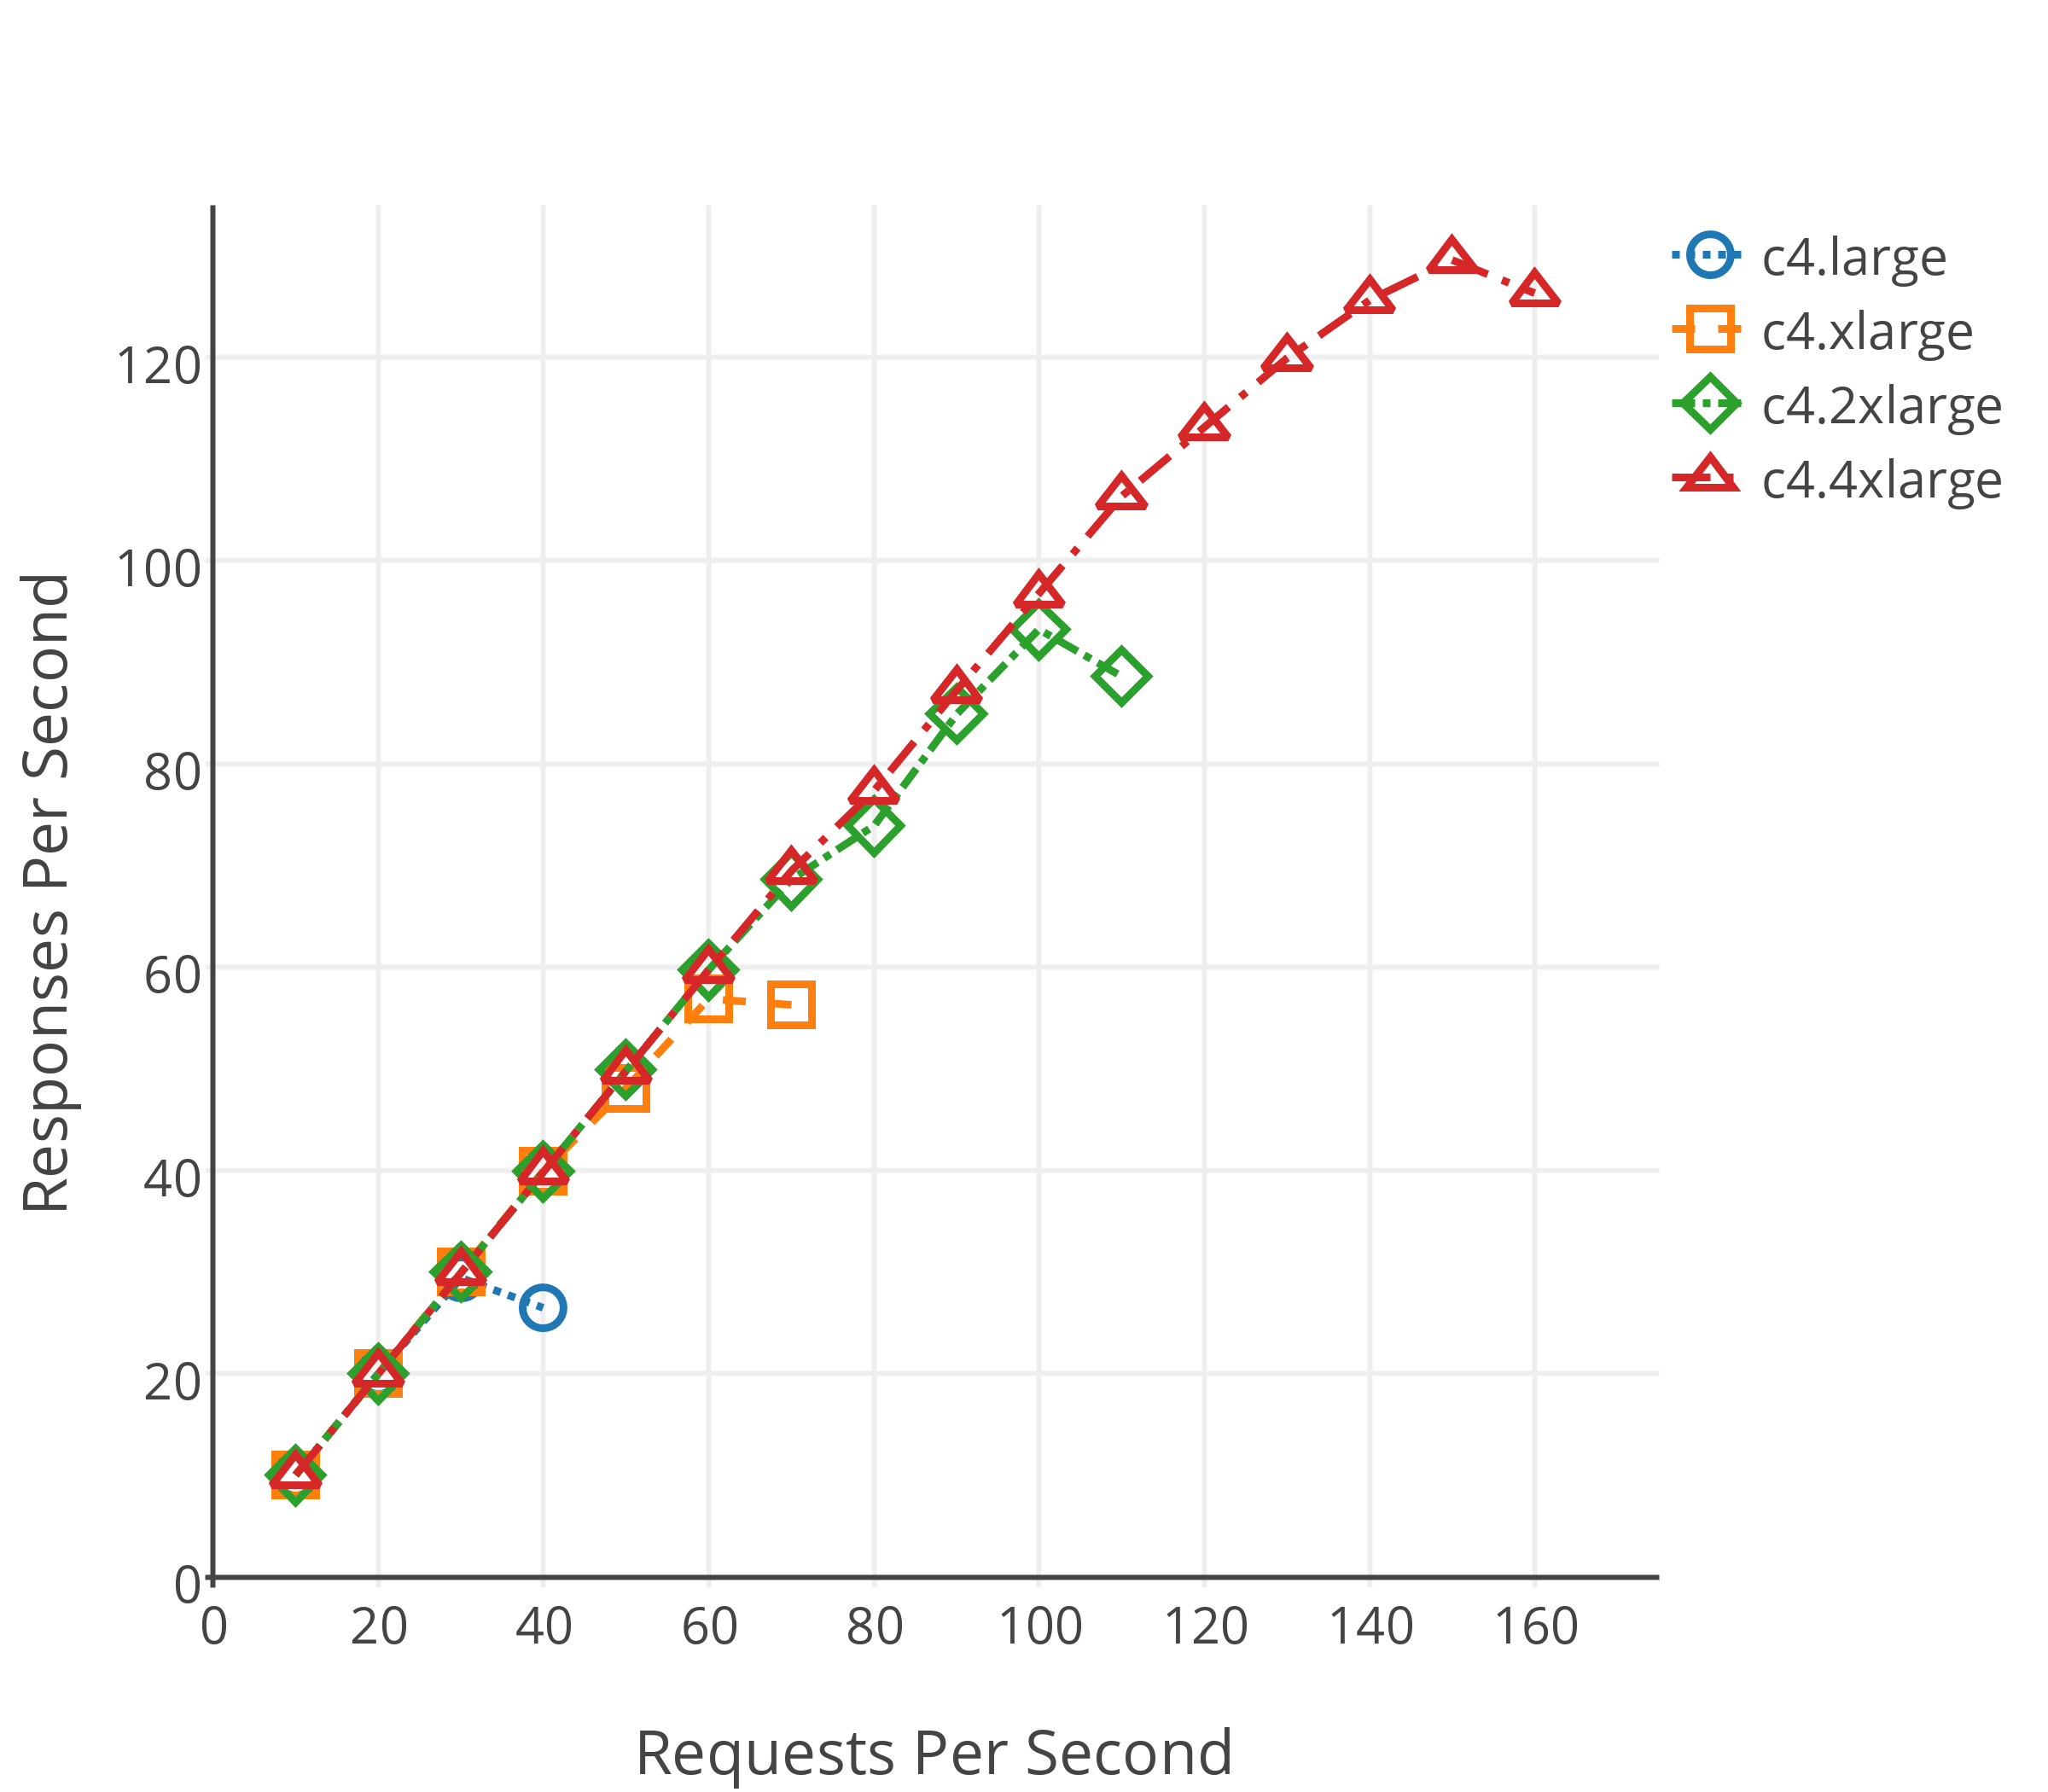
\includegraphics[width=\textwidth]{./figs/png/get_ac_auth_comp_chart.png}
    \caption{AC Server -- Get Authorization Token}
    \label{fig:eval:scaleup:gettoken}
  \end{subfigure}
  ~
  \begin{subfigure}[t]{0.48\textwidth}
    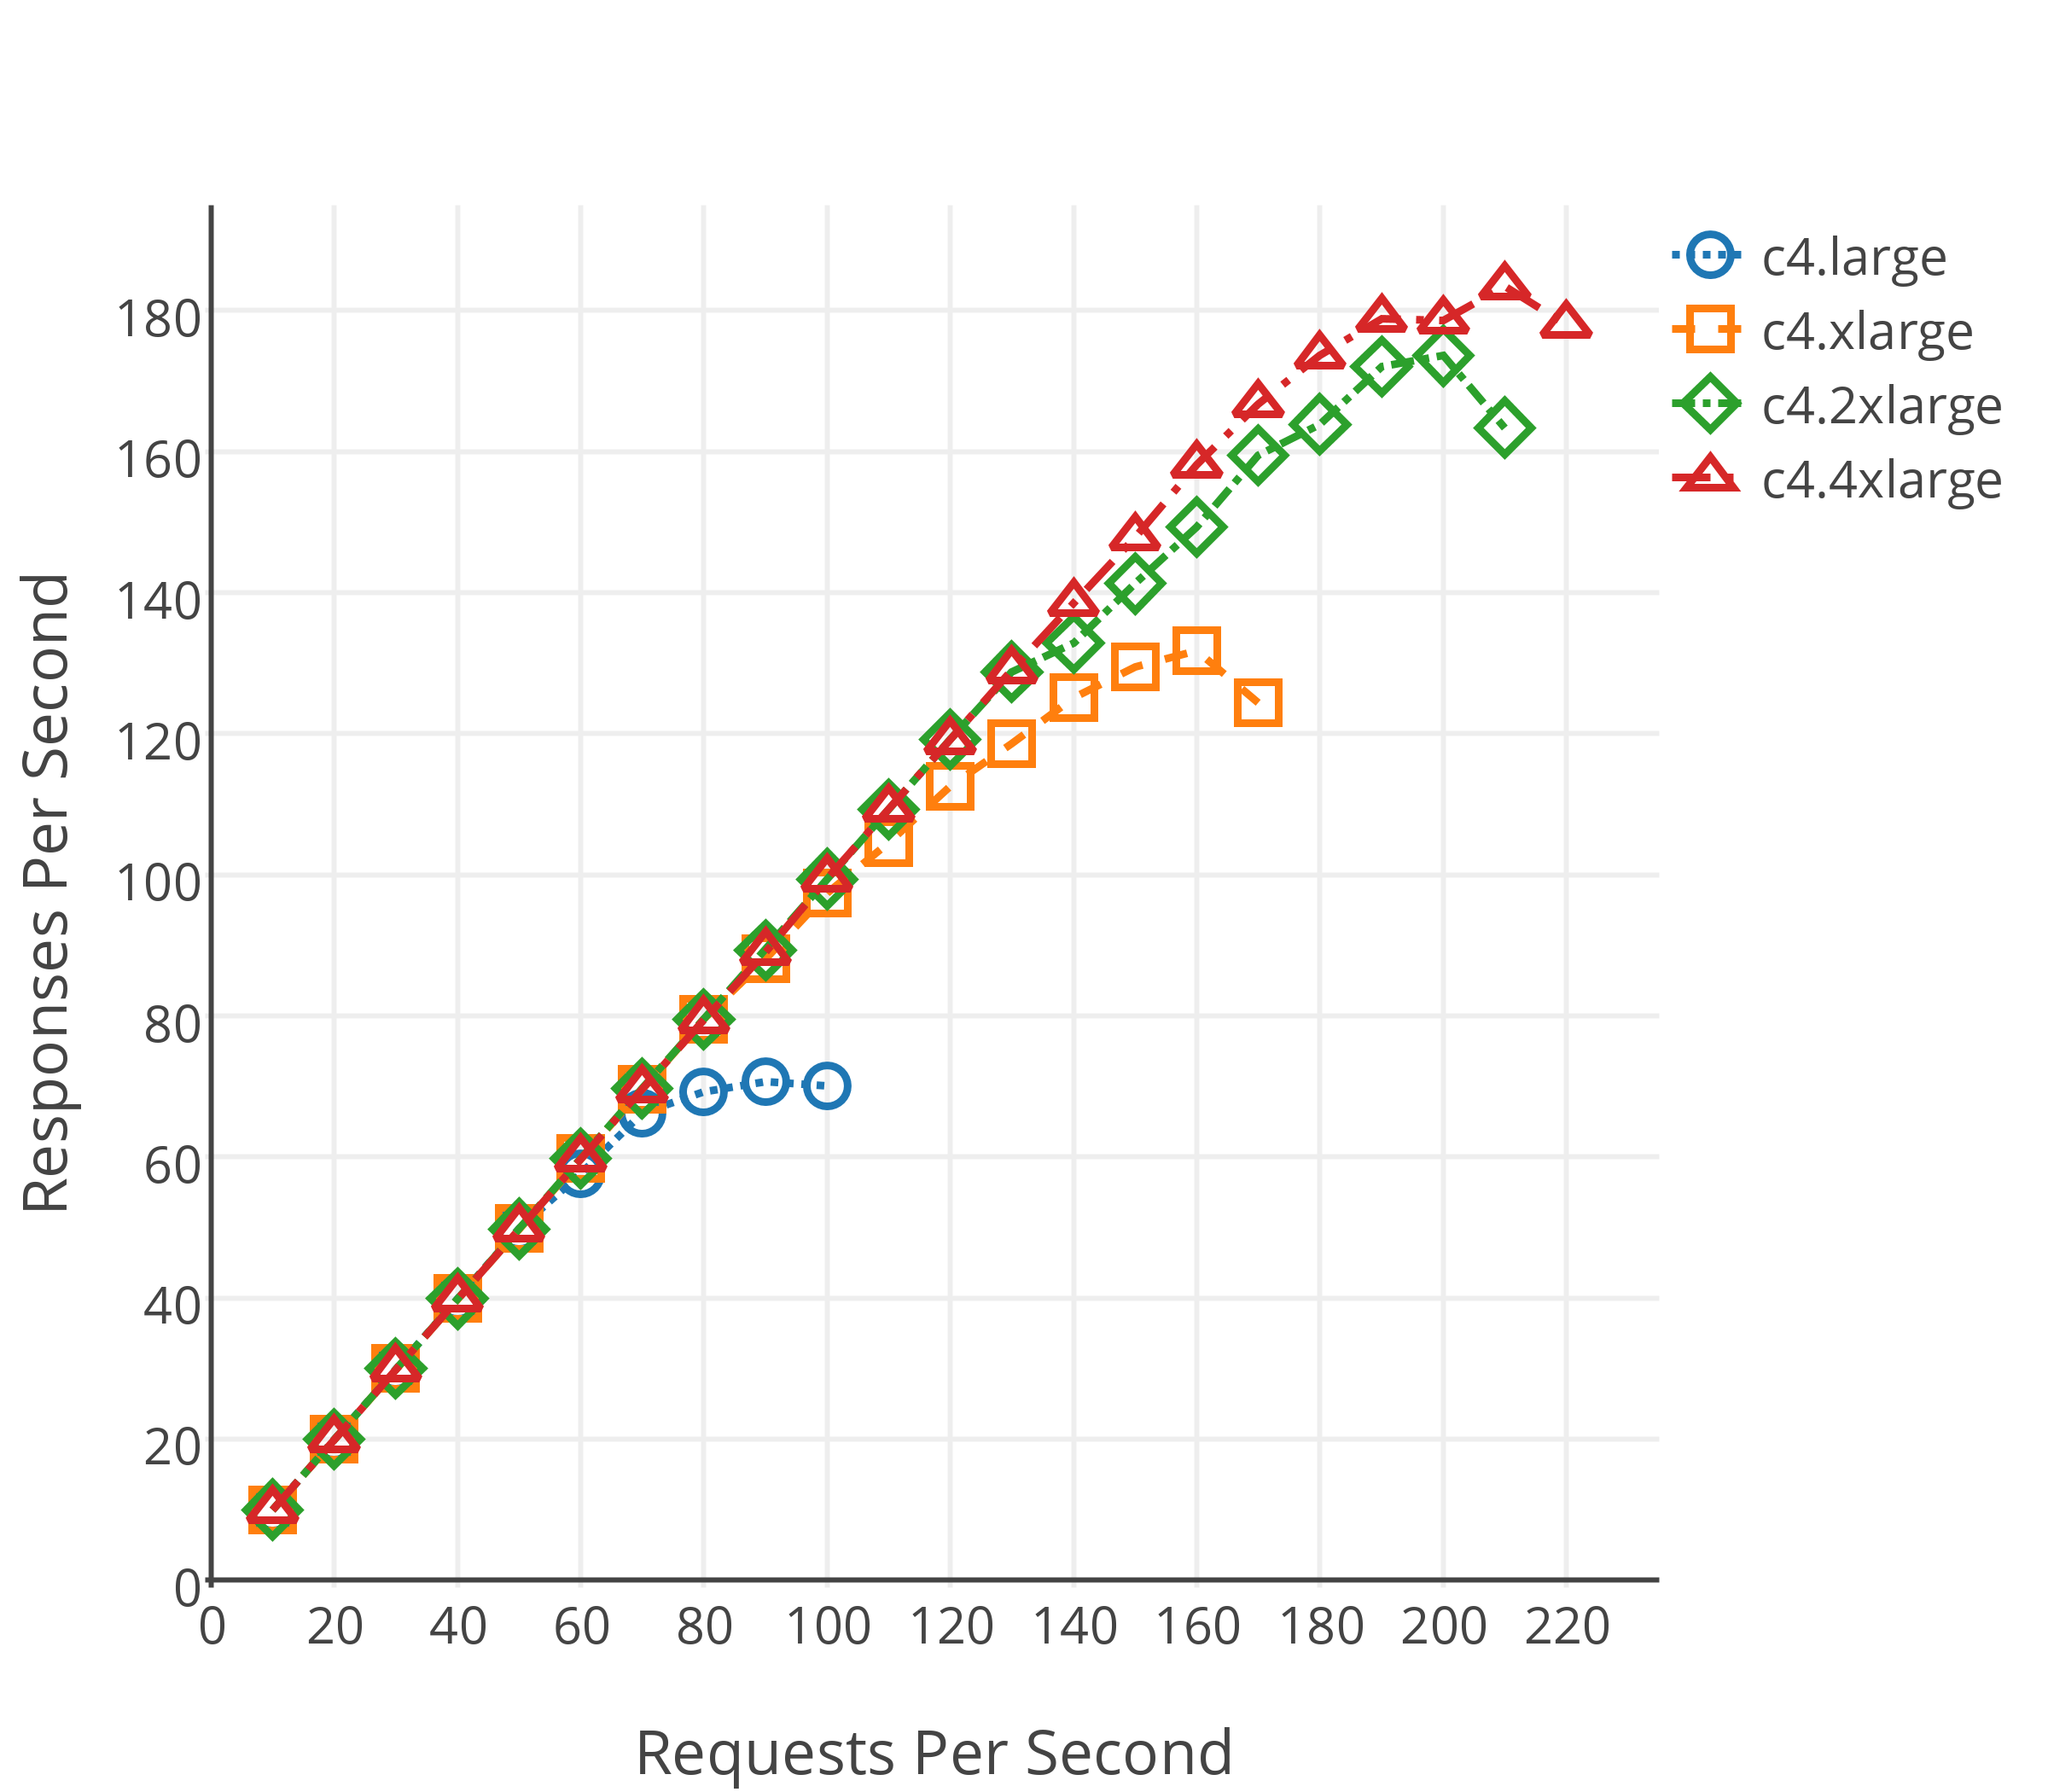
\includegraphics[width=\textwidth]{./figs/png/get_ss_secret_comp_chart.png}
    \caption{Storage Server -- Fetch Secret}
    \label{fig:eval:scaleup:getsecret}
  \end{subfigure}
  \caption{Scale Up Performance of Tutamen Servers on Amazon EC2
    Gen4 Compute-Optimized Instances}
  \label{fig:eval:scaleup}
\end{figure*}

Figure~\ref{fig:eval:scaleup} shows the response vs request rates of
both an access control and storage server deployment across a range if
increasingly powerful Amazon EC2 compute-optimized instances. The
response vs request curve for each instance tops out once the server
reach's its maximum processing capability. Increasing the request rate
beyond that point only serves to increase the response latency, and
eventually leads to diminished performance due to server
thrashing. Thus, we only graph through the first data point that shows
a decrease in response rate relative to previous data point, and this
that represents the asymptotic performance limit of each flavor.

Figure~\ref{fig:eval:scaleup:gettoken} shows performance of a stream
of ``Get Authorization Token'' requests to a single Tutamen Access
Control server for a verifier that requires only account membership
(e.g. no authenticator modules). As shown, the max request rate scale
fairly linearly with the number of CPU cores, ranging from topping out
around 30 RPS on a c4.large to topping out around 130 RPS on a
c4.4xlarge. Processing authorization token requests tends to be the
most computationally difficult Tutamen operation, as the process
requires verifying both cryptographic assertions (e.g. a client
certificate via the account ID) as well as loading and verifying each
authenticator module (where required). Such processing can also incur
human-scale delays far in excess of the computational limits, such as
in cases where an SMS authenticator is used requiring a human to
receive and then respond to a text message.

Figure~\ref{fig:eval:scaleup:getsecret} shows a similar set of curves
for a stream of request to fetch a secret from a Tutamen storage
server. As in the access control case, these operations scale linearly
with the number of CPU cores, up until the point where they start to
top out via the diminishing return of a c4.4xlarge instance relative
to a c2.2xlarge instance. While we have not fully determined the exact
cause of this limit, we believe it is a combining of our Python test
client itself being only capable of generating ~180 requests per second
and the fact that the Redis database starts to reach the limit of I/O
performance around this point, leading us to become I/O instead of CPU
bound. It should be noted that the request secret operation requires
significantly fewer computational resources than the ``get token'' operation,
leading to a performance range of ~70 RPS to ~180 RPS.

These data lead us to believe that Tutamen could be further scaled
both up (at least in the case of the Access Control server) and out
(e.g. by leveraging a load balancer and additional Tutamen server
backends sharing a common database cluster). Like other web-scale
server implementations, Tutamen is designed to allow both horizontal
and vertical scaling, and we foresee large deployments overcoming both
the computer and I/O barriers of our current deployment through a mix
of balancing requests across multiple backend instances and the use of
more powerful processing capabilities (e.g. the use of cryptographic
accelerators).

\begin{figure*}[th]
  \centering
  \begin{subfigure}[t]{0.48\textwidth}
    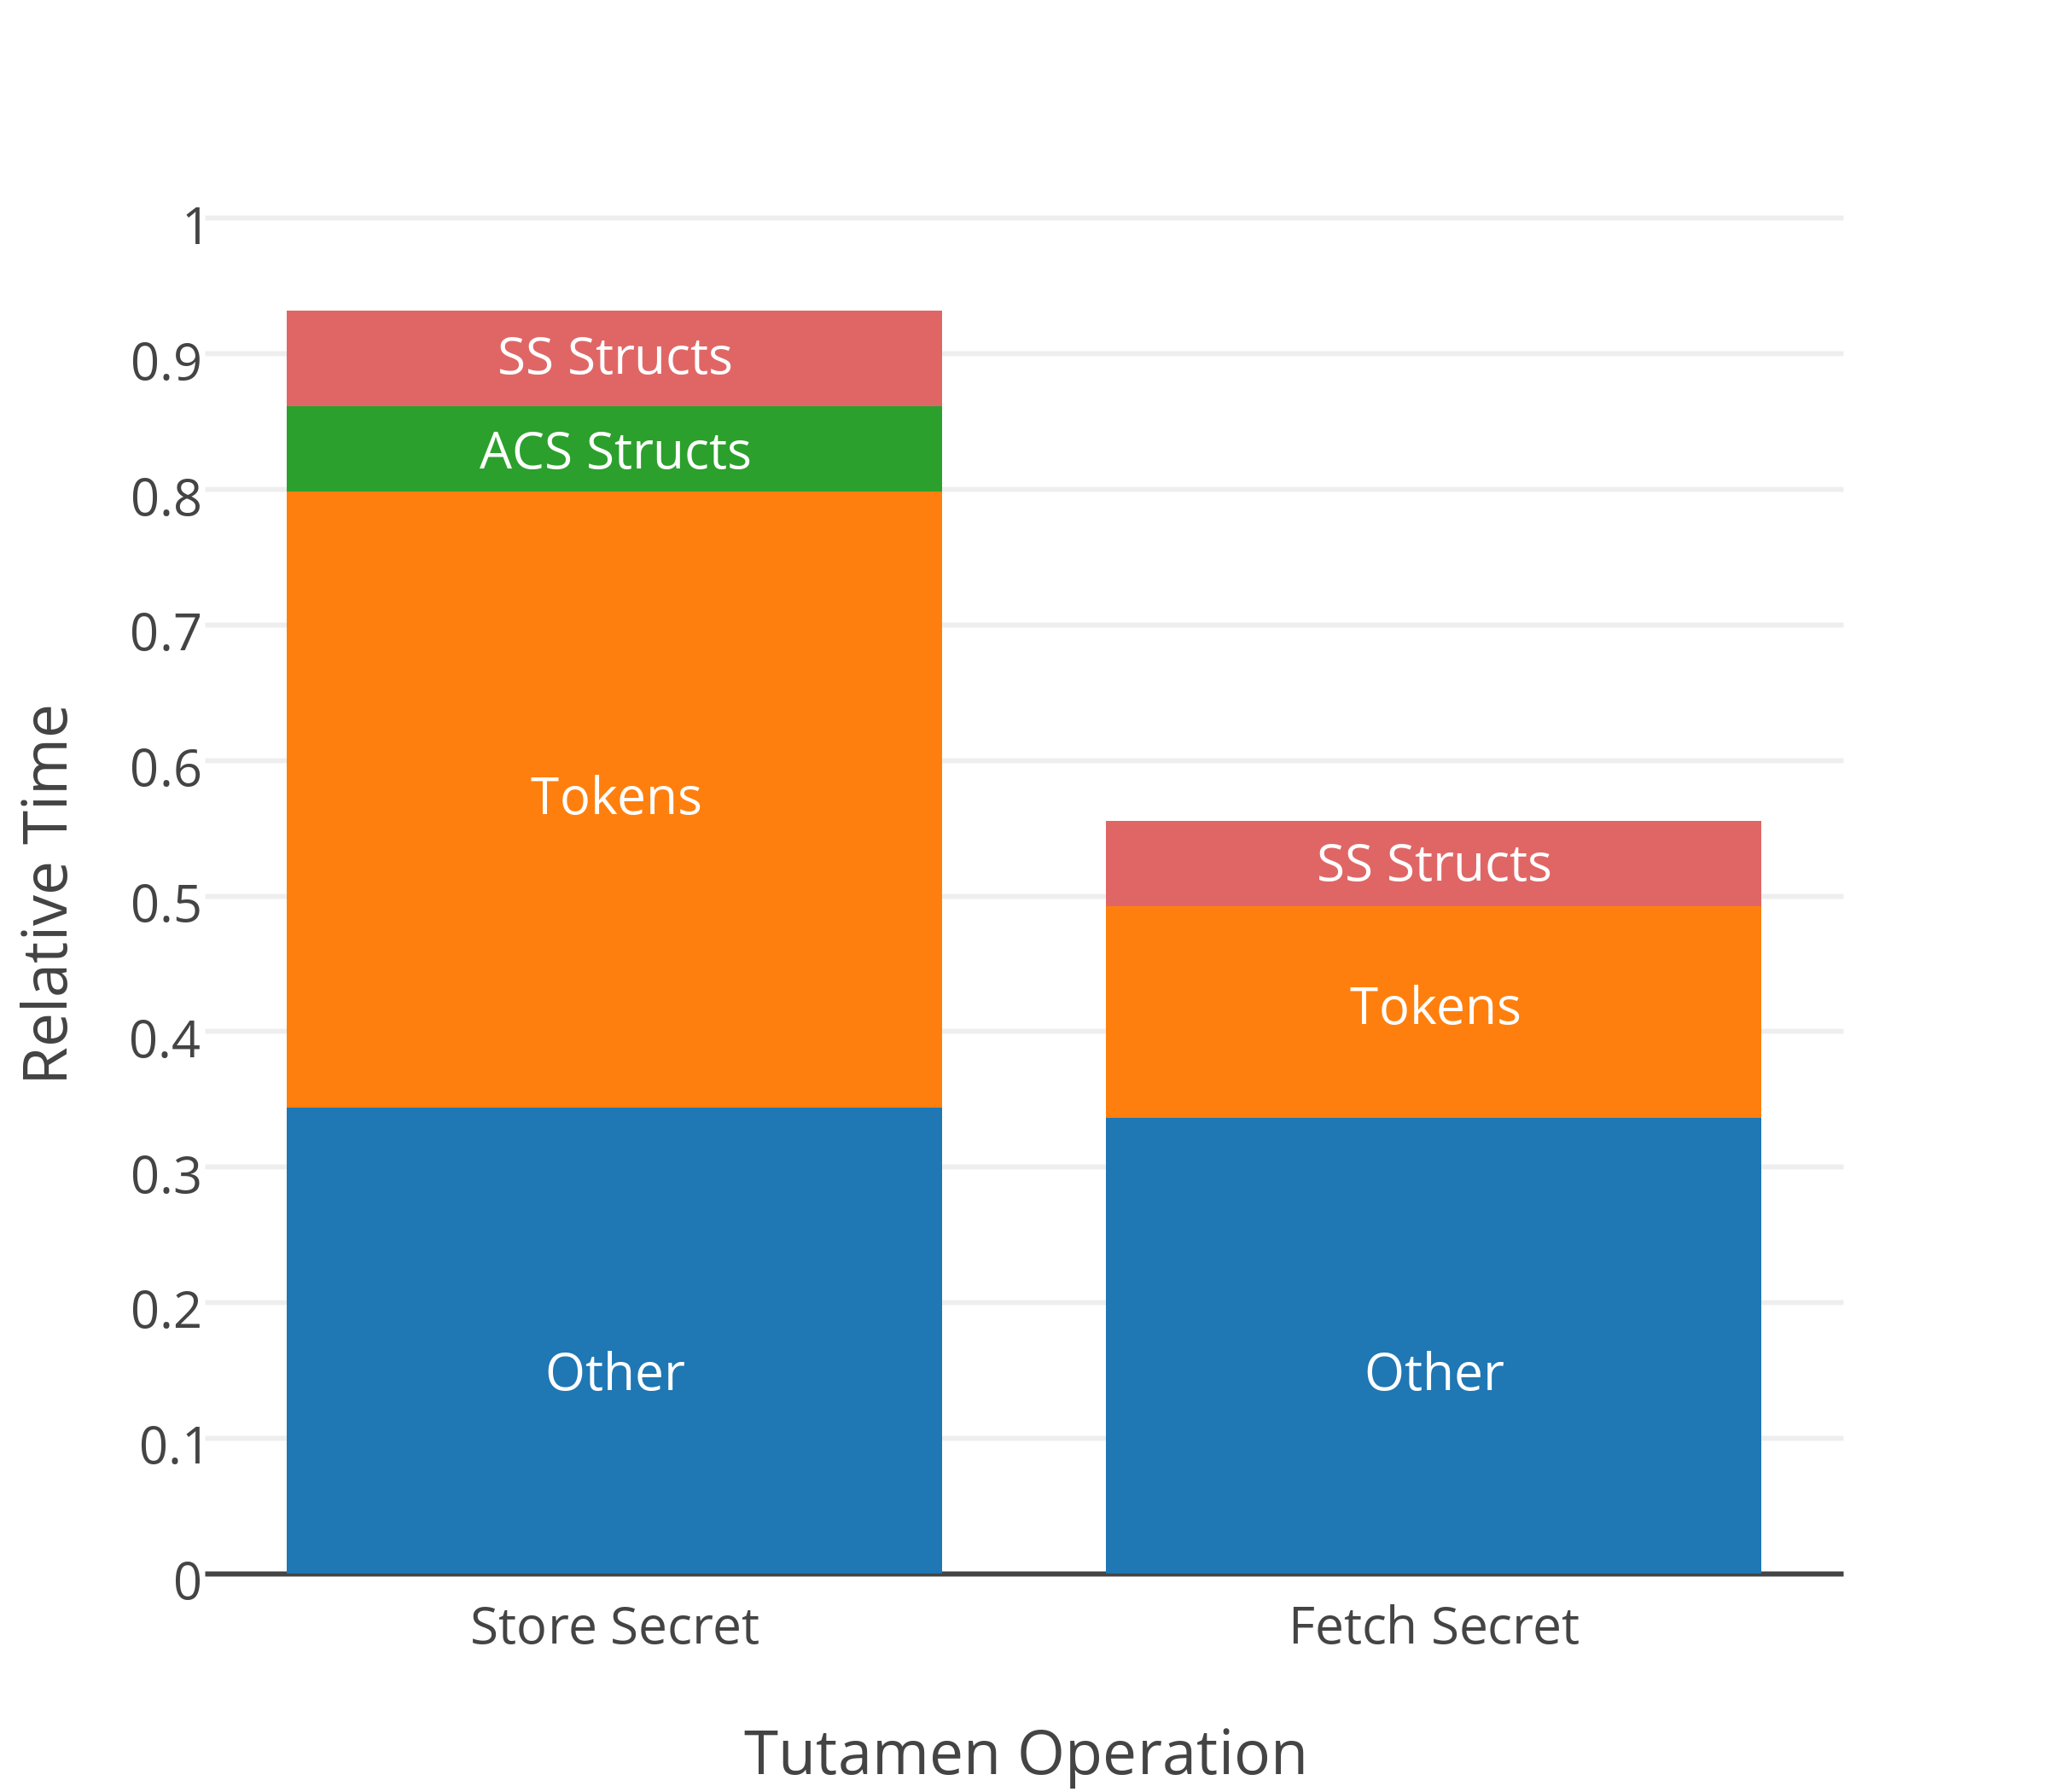
\includegraphics[width=\textwidth]{./figs/png/timing_bars_chart.png}
    \caption{Relative Time Spent Processing Store and Fetch
      Operations}
    \label{fig:eval:rel:secret}
  \end{subfigure}
  ~
  \begin{subfigure}[t]{0.48\textwidth}
    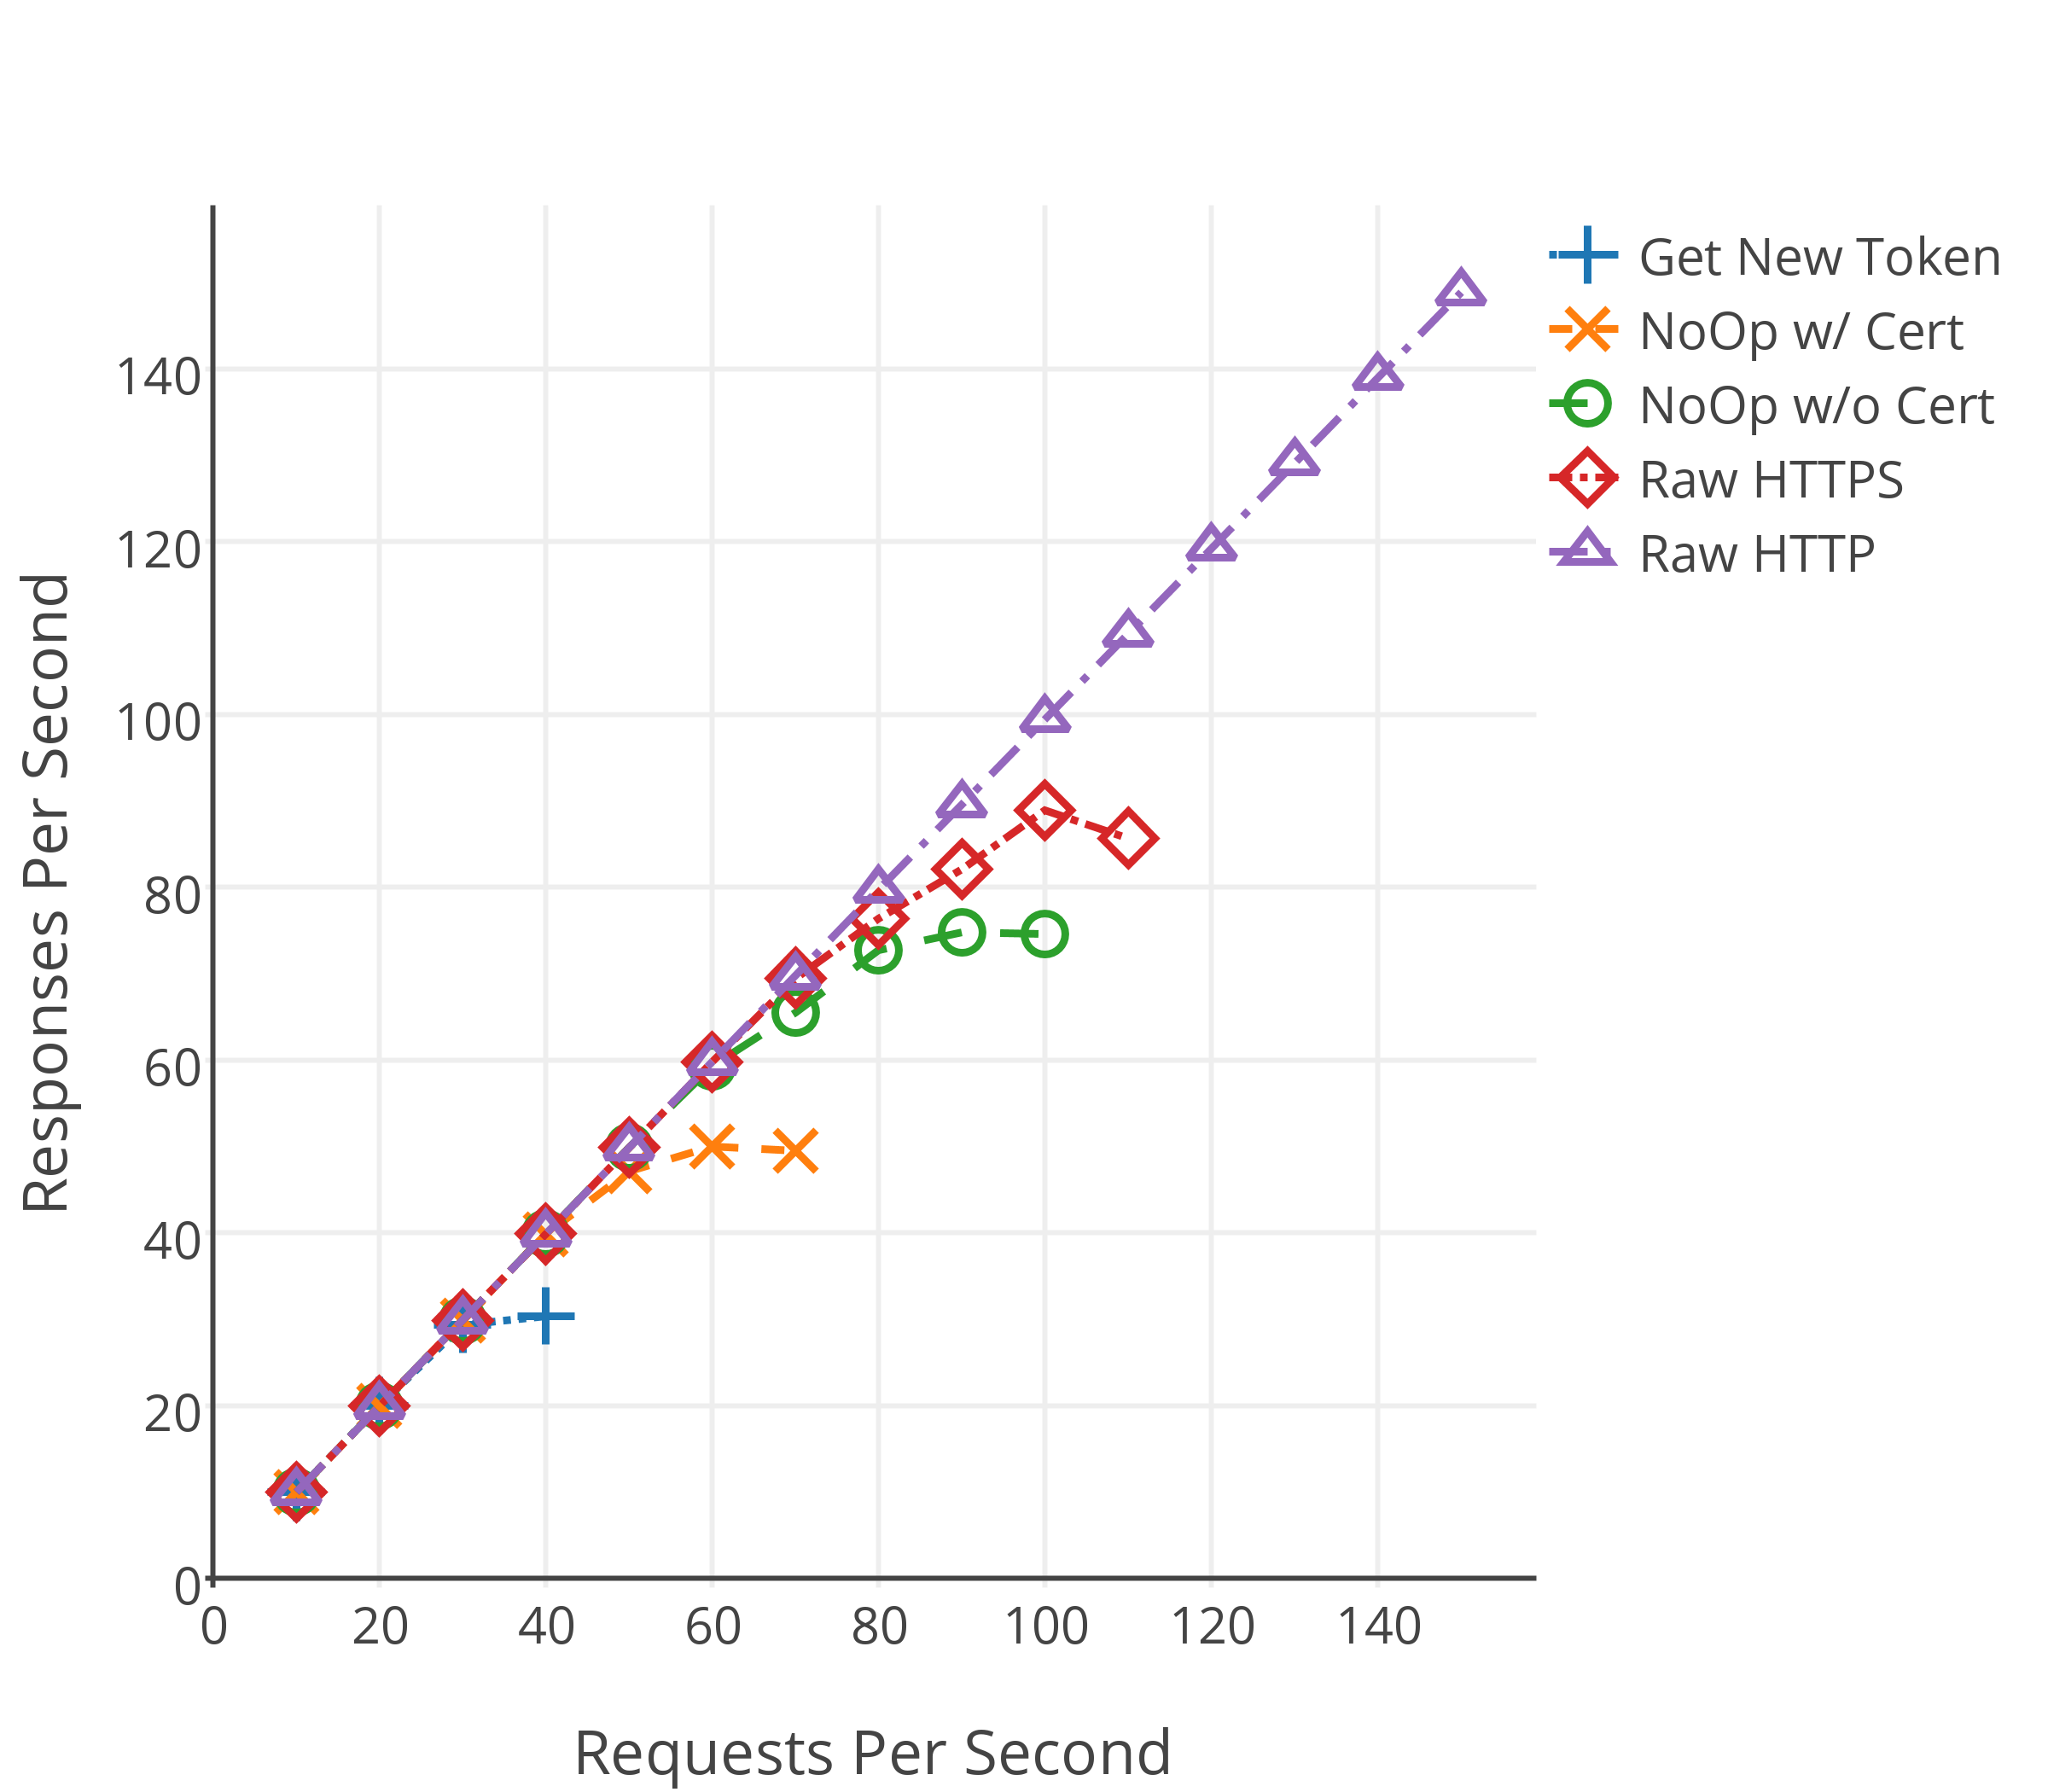
\includegraphics[width=\textwidth]{./figs/png/get_ac_auth_breakdown_chart.png}
    \caption{Relative Performance of Tutamen AC Server Operations}
    \label{fig:eval:rel:acops}
  \end{subfigure}
  \caption{Timing and Performance Comparison of Tutamen Server
    Operation Sub-components}
  \label{fig:eval:rel}
\end{figure*}

Figure~\ref{fig:eval:rel:secret} shows the breakdown of the relative
time required to complete two of the most common Tutamen operations:
storing a new secret and retrieving a previously stored secret. We
profiled the amount of time the Tutamen CLI application spent
performing various parts of each of these two Tutamen operations. In
both operations, the bulk of the server-related runtime is spent
requesting and retrieving the authorization tokens required to
complete the associated operations. In the secret creation case, five
tokens are required.\footnote{One token to create the permissions for
  a new verifier, one token to create a new verifier itself, one token
  to create permissions for a new collection, one token to create the
  collection itself, and one token to store a new secret within the
  collection.} In the secret read case, only a single token is
required.\footnote{One token to read a secret within the collection.}
The remainder of the server-related time is spent either creating AC
and storage data structures (e.g. verifiers, collections, etc), or
reading existing data structures. The ``other'' time is spent reading
the Tutamen config files, loading the necessary client certificates,
and dealing with the overhead required to setup the TLS connections
and interpret the Python-based CLI.

It is not unexpected that the client must spend the bulk of its time
requesting tokens and waiting for them to be approved -- token
verification is the primary role the access control server must
perform, and depending on the complexity of the verifiers associated
with the permission the token is requesting, verification can be a
fairly complex task. When performing these measurements, we employed a
simple verifier that only required client membership in a specific
account. Verifiers that include human-in-the-loop authenticators
(e.g., SMS approval) would increase the token turnaround time by the
amount of time the human requires to provide approval. To help
alleviate these waits on applications that must perform a high number
of Tutamen requests, Tutamen tokens may be reused up until their
expiration time. Thus, it is possible for an application to request a
long-lived token and to reuse this token to access multiple secrets
within the collection to which the token grants read access.
 
Figure~\ref{fig:eval:rel:secret} shows the response vs request rate
for a standard token request operation, two ``No-Op'' AC API
operations (one that sends and verifies the client TLS certificate and
one that does not), and raw Apache HTTPS and HTTP page loads as
preformed on an Amazon EC2 c4.large instance. As these curves show,
token verification on such an instance tops out around 30 RPS. The
null AC API operation with client certificates tops out around 50 RPS,
and the null operation without client certificates tops out at about
75 RPS. Raw HTTPS tops out around 90 RPS. HTTP topped out around 550
rps (curve truncated for viewability). Out Tutamen prototype is thus
primarily limited by the TLS overhead required to serve the
application and verify client certificates. Token verification itself
also incurs additional computational requirements, including
cryptographic signing operations. Finally, the data retrieval itself
incurs some overhead. Given the cryptographic limits of the current
prototype, we have plans to increase the performance of single Tutamen
server by both streamlining the cryptographic processing code and by
employing hardware-based cryptographic/TLS accelerators. These
technique, coupled with plans to further optimize the data retrieval
path and the scale up and scale out capabilities discussed previously
lead us to believe that Tutamen can be grown to support much larger
numbers of operation and users with only moderate additional
efforts. The Tutamen server code could also be converted into a
compiled language (e.g. golang~\cite{golang}) to avoid the overhead
imposed by using an interpreted language.

%%  LocalWords:  Tutamen Tutamen's verifiers authenticators SMS Xeon
%%  LocalWords:  authenticator HTTPS Redis viewability Scaleway QCOW
%%  LocalWords:  FuseBox xlarge CPUs golang
